%% PHYSICS:
\documentclass[submission, Phys]{SciPost}

% Prevent all line breaks in inline equations.
\binoppenalty=10000
\relpenalty=10000

\hypersetup{
    colorlinks,
    linkcolor={red!50!black},
    citecolor={blue!50!black},
    urlcolor={blue!80!black}
}

\usepackage[bitstream-charter]{mathdesign}
\urlstyle{sf}

% Fix \cal and \mathcal characters look (so it's not the same as \mathscr)
\DeclareSymbolFont{usualmathcal}{OMS}{cmsy}{m}{n}
\DeclareSymbolFontAlphabet{\mathcal}{usualmathcal}

\begin{document}

% The article title is centered, Large boldface, and should fit in two lines
\begin{center}{\Large \textbf{
Domain Wall Dynamics for a 1D Bose gas\\
}}\end{center}

% TODO: write the author list here. Use first name (+ other initials) + surname format.
% Separate subsequent authors by a comma, omit comma and use "and" for the last author.
% Mark the corresponding author with a superscript star.
\begin{center}
Léa Dubois\textsuperscript{1}, G. Themèze, J. Dubail and I. Bouchoule,
% Aah B. Cee\textsuperscript{1} and
% Gee K. See\textsuperscript{2$\star$}
\end{center}

% TODO: write all affiliations here.
% Format: institute, city, country
\begin{center}
{\bf 1} Laboratoire Charles Fabry, Institut d'Optique, Université Paris-Saclay
% \\
% {\bf 2} Affiliation2
% \\
% {\bf 3} Affiliation2
\\
% TODO: provide email address of corresponding author
${}^\star$ {\small \sf lea.dubois@universite-paris-saclay.fr}
\end{center}

\begin{center}
\today
\end{center}

% For convenience during refereeing (optional),
% you can turn on line numbers by uncommenting the next line:
%\linenumbers
% You should run LaTeX twice in order for the line numbers to appear.

\section*{Abstract}
{\bf
Abstract
}


% Guideline: if your paper is longer that 6 pages, include a TOC
% To remove the TOC, simply cut the following block
\vspace{10pt}
\noindent\rule{\textwidth}{1pt}
\tableofcontents\thispagestyle{fancy}
\noindent\rule{\textwidth}{1pt}
\vspace{10pt}

List of figures  : 
\begin{itemize}
    \item For the experimental setup : atom chip with the shape of the longituinal trap + linear density profil of the initial situation
    \item For the experimental data : Euler scale observed
    \item For the experimental data : edge profile with (T=0, Lieb-Liniger) and (T=0, GP) 
    \item experimental edge profile + fit by GE + fit of the left part by GE + fit of the right part by GE + insert avec fig. 9.9 de la thèse de Léa 
    \item (a) experimental edge profile + fit by  function s (4 fittng parameters) ; (b) distribution des facteurs d'occupation (c) distributions de rapidités
    %\item Non thermal ansatz : Thermal and non thermal occupation factor (and rapidity distribution ???) + superposition with the experimental profile.
    \item  local rapdity distribution : voir dernière figure déjà mise 
\end{itemize}

\section{Introduction} 
%[Permier jet : Isabelle]
\label{sec:intro}

 Gaining insight on the out-of-equilibrium dynamics of many-body quantum systems is  the tremendously difficult and it is the goal of an active research field.  
One particular class of systems where important progress have been done is the class of integrable one-dimensional systems. 
%In contrast to ergodic systems 
%which relaxe, as long as local observable are concerned, towards thermal states parametrized by a few quantities, the quilibrium states which emerge after relaxtion in intergable systems are parametrised by a whole function, their rapidity distribution[]. 
Owing to their infinite number of local conserved charges, to describe the local properties of equilibrium states,  that arrise after relaxation, one needs a  whole function, the rapidity distribution[]. 
The latter can be viewed as the distribution in velocity space 
of the infinite-lifetime quasi-particles in the system. Large scale dynamics is 
accounted for by a generalized hydrodynamic (GHD) effective theory[], which 
assume local equilibrium.
A paradigmatic situation that can be handled by  this theory is the dynamics 
induced by a partite quench\cite{bertini_transport_2016,castro-alvaredo_emergent_2016}, dubbed  domain-wall protocol in this paper. In this protocol the Hamiltonian governing the  dynamic is translation 
invariant but the initial state is the junction of  two-semifinite 
homogeneous systems prepared each in a different equilibrium state of the Hamiltonian. The GHD theory predicts that, at time long enough such that diffusion effects become negligible\cite{de_nardis_diffusion_2019} and Euler-scale hydrodynamics is valid,  the time evolution is ballistic. % and the local state a time $t$ after the junction and at a position $x$ from the merging point is solely a function of $x/t$. 
An interesting feature of this protocol is that the local state, within the merging region, is expected to presents features
caracteristic of zero-temperature systems. Thus this protocol could be used to reveal power-law singularities of correlation function characteristic of zero-temperature Luttinger liquid\cite{de_nardis_edge_2018}, providing a local  probe is performed. 

In this paper, we experimentally realize an instance of the domain-wall protocol
using an ultra-cold atomic Bose gas, well described by the Lieb-Liniger model of 
one-dimensionnal Bosons with contact repulsive intercations\cite{lieb_exact_1963,bouchoule_generalized_2022}, which is an integrable model. 
The domain wall consists in our experiment in the junction of a gas prepared in an equilibrium state on the one side, and the vaccuum on this other side. It is prepared starting from an homogeneous cloud, by the sudden removal of its left part. For different evolution times, we record the density profile of the border between the two zones, dubbed the border profile. We find that the border profile shows a ballistic behavior, as expected from GHD theory at Euler scale. 

The border profile, for clouds prepared with deep evaporative cooling, is in fair agreement with GHD predictions assuming the semin-inifite gas is in its ground state, altgough deviations are present. We show that, from the border profile, it is in principle possible to reconstruct the rapidity distribution characterising the initial gas. This protocol can thus be used as a generalized thermometry. 
However, the reconstruction method suffers from a high sensitivity to experimental noise in the tail of the border profile which prevent us to reconstruct faithfully the initial rapidity distribution. Instead we use anstaz parametrized by a few parameters to extract the rapidity distributions of the initial gas from a fit to the border profile. 

Finally, we use a newly developed techniques\cite{dubois_probing_2024} to probe the local rapidity distribution within the border. The latter is expected to be highly asymetric for an initial state whose rapidity distribution is substantially broader and 
smoother than that of the ground state:  while one of its border 
reflects the broad character of the initial rapidity distribution, the other border 
present the sharp feature expected for the ground state.  Our expereimental data show such an asymetric behavior, although the above feature is softened by the finite spatial resolution of the local rapidity distribution measurement.  
%\begin{itemize}
%    \item Introducing GHD to introduce the protocol : introducing the problem in terms of rapidity distribution and in terms of occupation factor.
%\end{itemize}


\section{Experimental setup}
{\bf [Premier jet : Léa]}
\subsection{Atom chip experiment}
\begin{itemize}
    \item Explain that the shape of the longitudinal potential locally at the center of the chip can be developed in polynomials. We can restrict ourselves to the first 4 predominant terms such as the potential is writen $V(x) = \sum_{i=1}^{4} a_i x^i$. Each coefficient $a_i$ can be adjusted by changing the currents flowing through the four wires that generate the longitudinal potential.
\end{itemize}

\subsection{Producing a initially semi infinite homogeneous 1D Bose gas}

\begin{figure}[!htb]
    \centering
    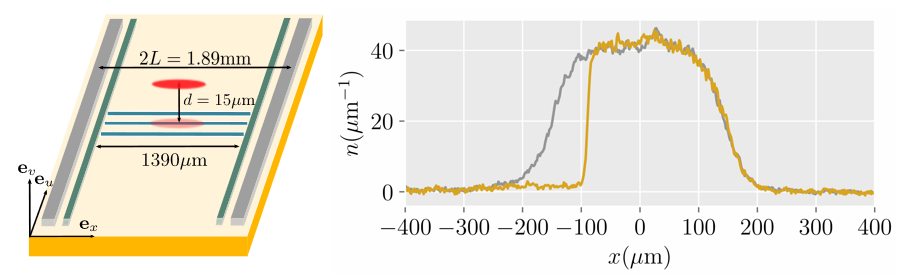
\includegraphics[width=1.0\linewidth]{Figures/Atom_chip.PNG}
    \caption{(a) $-$ (b) The grey curve represents the linear density profile of gas confined within a quartic potential. The atomic cloud is then illuminated during $30 \mu$s by a near resonant light beam, shaped using a DMD. The resulting density profile is depicted in yellow.}
    \label{fig:enter-label}
\end{figure}

\section{GHD predictions}
%{\bf [Premier jet : Isabelle]}
Upon time evolution, the initial sharp border of the cloud broadens and time
derivative of local quantities decrease. 
After some time, %Once its extension is large compared to microscopic length scales, 
upon coarse graining in position an time, one expects that the gas can locally be described by equilibirum states.
%is locally in equican 
%describe the system in terms of its local rapidity distribution $\rho(x,t,\theta)$. %We denote $\rho(x,t,\theta)$ the rapidity distribution at position $x$ and time $t$, which fulfills $\int d\theta \rho(x,\theta) = n(x,t)$ where 
%$n$ is the linear atomic density. 
Equilibrium states of the Lieb-Liniger model are entirely characterized 
by their rapidity distribution $\rho(\theta)$.
Equivalently, equilibrium states can be parametrized by  a function $\nu(x,t,\theta)$ dubbed the occupation factor distribution which takes values between 0 and 1 and which is related to  
$\rho$ by $\nu(\theta)=\rho(\theta)/\rho_s(\theta)$, where $\rho_s(\theta)=
1/(2\pi) \left (1+ \int d\theta' \Delta(\theta-\theta') \rho(\theta')\right ) $
and the function $\Delta$ is $\Delta(\Theta)=2g/(g^2/\hbar+\hbar\Theta^2)$. 
 The functions $\nu$ and $\rho$ are in one-to-one correspondance and in the following we use either $\rho$ or $\nu$. 
Since local equilibrium is assumed, the system as a whole is described by a time and position dependent rapidity distribution $\rho(x,t,\theta)$ or equivalently by the 
occupation factor distribution $\nu(x,t,\theta)$. The former is particularly usefull to extract the linear density, which reads $n(x,t)=\int d\theta \rho(x,t,\theta)$.
%Equivalently, one can describe the system locally with a function $\nu(x,t,\theta)$ which takes values between 0 and 1 and dubbed the occupation factor distribution.  This function is related to  
%$\rho$ by $\nu(\theta)=\rho(\theta)/\rho_s(\theta)$, where $\rho_s(\theta)=
%1/(2\pi) \left (1+ \int d\theta' \Delta(\theta-\theta') \rho(\theta')\right ) $
%and the function $\Delta$ is $\Delta(\Theta)=2g/(g^2+\Theta^2)$. 
%The functions $\nu$ and $\rho$ are in one-to-one correspondance and in the following we use either $\rho$ or $\nu$. 
%$\nu$ takes its value in $[0,1]$. 
%The state of the system can equivalently be represented by


The GHD theory provides a prediction for
the time-evolution of $\rho$, or equivalently of $\nu$. At large enough length scales, it reduces to its Euler-Scale approximation which, written in terms of $\nu$, takes the convective form 
\begin{equation}
\frac{\partial\nu}{\partial t} + v^{\rm{eff}}_{[\nu]}\frac{\partial  \nu }{\partial x} = 0
\end{equation}
where the effective velocity $v^{\rm{eff}}_{[\nu]}$ is a functional of the local rapidity distribution which fulfills, for any rapidity $\theta$,
%\begin{equation}
$v_{[\nu]}^{\rm{eff}}(\theta) = \theta -\int \frac{d\theta'}{2\pi} \Delta(\theta-\theta'') \rho(\theta')\left (  v_{\rm{eff}}(\theta) - v_{\rm{eff}}(\theta') \right )$.
%\end{equation}
%where $\Delta(u)=2g/(g^2+u^2)$.  
%This equation, together with the initial domain wall initial state, is invariant
For an initial domain-wall state whose discontinuity is located on $x=0$, the solution of \eqref{eq:ghd} is invariant along rays of constant velocity $x/t$ and we indroduce the occupation factor distribution of the rays $\nu^*(v,\theta)$ such that 
\begin{equation}
\label{eq:nuvsnuetoile}
    \nu(x,t,\theta)=\nu^*( x/t,\theta).
\end{equation} 
This equation implies that all local properties of the gas depend on $x$ and $t$ only through the quantity $x/t$. 
For the domain wall situation considered in this paper with, initially, a  vaccum state for negative $x$ and 
a state of occupation factor distribution $\nu_0$ one the right, 
 the function $\nu^*(v,\theta)$ is parametrised by an edge rapidity $\theta^*$ according to
\begin{equation}
\label{eq:nuetoile}
    \nu^*(v,\theta)=\left \{ \begin{array}{l} 
    \nu_0(\theta) \mbox{ if } \theta < \theta^*\\
    0 \mbox{ if } \theta > \theta^*\\
    \end{array} \right . \mbox{ where  }  v^{\rm{eff}}_{[\nu^*]}(\theta^*)=v.
\end{equation}
%where $\theta^*$ is such that $v^{\rm{eff}}_{[\nu^*]}(\theta^*)=v$.
This equations can be solved numerically 
if the initial distribution $\nu_0(\theta)$ is known. Together with Eq.\eqref{eq:nuvsnuetoile}, it entirely describes the system after the Euler-scale has been 
reached. Note that to compute the linear density $n(x,t)$ in order to compare to experiments,  one
uses the relation $n(x,t)=\int d\theta \rho(x,t,\theta)$, such that the rapidity distribution
needs to be computed from the knowledge of $\nu(x,t,\theta)$.

\paragraph{Solution for a system initially in the ground state.}
As an example, let us derive some implications of the above equations in the case the  initial state is the ground 
state. The initial occupation factor distribution is then a Fermi sea. More precisely $\nu_0(\theta)=1$ if $|\theta| < \theta_m$ and zero otherwise, where the fermi radius $\theta_m$ depends on the initial linear density $n_0$. 
Some general features of the state of the system after the 
Euler-scale has been reached can be identified. The border has well defined  
fronts both in the empty region of $x<0$ and in the region of density
$n_0$ for $x>0$. In the region $x<0$, the front is at 
$x/t =\theta_m$, since the effective velocity of a vanishingly narrow fermi sea is equal to its mean rapidity. The density vanishes for $x/t<-\theta_m$. In the region $x>0$, the front is at $x/t = c$, where $c=v^{\rm eff}_{[\nu_0]}(\theta_m)$ is the speed of sound for the density $n_0$. For $x/t>c$, the system is not yet affected by the border deformation.  Finally, for any $x/t$, the local state is a  fermi sea, displaced by some quantity $v(x/t)$ in rapidity space, which corresponds to a local galilean boost of velocity $v(x/t)$.
Exact solution can be derived  in the two asymptotic regimes
large and small densities. 

%In the hard core limit $\gamma=g/n_0\gg 1$, Eq.\eqref{} are easily solved using the fact that, in this regime , $v^{\rm eff} (\theta)=\theta$ and the intial fermi sea has a  radius $\theta_m \simeq \pi \hbar n_0/m$. The density profile of the border is then  computed using the fact that in this regime $\rho(\theta)=\nu(\theta)/(2\pi)$, and we obtain, within the border region 
%$|x|/t < \pi \hbar n_0/m$,
In the hard core limit $\gamma=g/n_0\gg 1$, Eq.\eqref{eq:nuetoile} is easily solved using the fact that, in this regime, $v^{\rm eff} (\theta)=\theta$ 
regardless of the occupation factor distribution. We then use Eq.\eqref{eq:nuvsnuetoile} and the fact that  a fermi sea of radius $\theta_m$ corresponds to a linear density $n=m\theta_m/(\pi\hbar)$ in this regime to derive 
\begin{equation}
    n(x,t)=\frac{n_0}{2} \left ( 1 + \frac{x}{t} \frac{m}{\pi \hbar n_0} \right ).
\end{equation}
We recover the results expected for a gas of free fermions, as expected from the mapping of the hard-core bosons to fermions, which presereves the density\cite{girardeau_relationship_1960}. 


%In the quasi-BEC regime $\gamma=g/n_0\ll 1$, the 
%fermi radius of the ground state 
%is $\theta_m \simeq 2\sqrt{mgn_0}/\hbar$. Then using several properties 
%specific to this regime, we can solve Eq.~\eqref{} and derive
%the density profile of the border which reads, in the border region 
%$-2\sqrt{mgn_0}/\hbar<x/t < \sqrt{mgn_0}/\hbar$,
In the quasi-BEC regime $\gamma=g/n_0\ll 1$, we sole Eq.~\eqref{eq:nuetoile} using the fact in this regime that the effective velocity at the border of a Fermi sea of radius $\theta_m$ is 
$\theta_m/2$, in the frame where the Fermi sea is at rest. Then, using Eq.\eqref{eq:nuvsnuetoile} and the fact that, in this regime, a fermi sea of radius $\theta_m$ corresponds to a linear density $n=m\theta_m^2/(4 g)$, we obtain
\begin{equation}
    n(x,t)= \frac{n_0}{9}\left ( \frac{x}{t}\frac{\hbar}{\sqrt{mgn_0}} +2 \right )^2  .
\end{equation}
We recover here the hydrodynamic predictions derived from the Gross-Pitaevski equation\cite{el_decay_1995,xu_dispersive_2017}, as exepcted since this classical field approach be a good description of the system in this regime. 

%The asymptotic behaviors of the fermi raduis for large and small densities are known:  
%for an interaction parameter $\gamma=g/n_0\ll 1$, {\it i.e.} in the qBEC regime, $\theta_m \simeq 2\sqrt{mgn_0}/\hbar$, while for $\gamma=g/n_0\gg 1$, {\it i.e.} in the hard-core regime, $\theta_m \simeq \pi \hbar n_0/m$.

%Once $\nu^*(v,\theta)$ is 
%known, the density profile $n(x,t)$ is easily obtained using Eq.\eqref{:} and it reads
%\begin{equation}
 %   n(x,t)=\int d\theta \nu^*(x/t,\theta).
%\end{equation}

%such that the rapidity distribution is 
%After a transiant time, on expect the Assuming spatial variation occur on 
%\subsection{Euler scale}
%\begin{itemize}
%    \item Change variable
%    \item Note that the Euler scale is not valid for short times. The spatial variations of the system are indeed not enough big compared to the characteristic microscopic lengths. However, effects beyond the Euler scale at short times become negligible for long dynamic times.
%\end{itemize}

%\textit{Transition :} 

%\subsection{Ground state}
%\begin{itemize}
%    \item Say that in the ground state the rapidiy distribution depends only on the Lieb parameter, which is then also the case for the edge deformation profile.
 %   \item Case $\gamma \to 0$
 %   \item Case $\gamma \to  \infty$
%\end{itemize}

\section{Experimental data}
{\bf [Premier jet : Léa]}
After preparing the initial state, the longitudinal confinement is removed while the transverse confinement is maintained to study the one-dimensional dynamics. The edge density profiles for different evolution times are shown in Fig.\ref{fig:euler} and represented in function of $x /\tau$. The profiles overlap remarkably well, the ballisitic evolution expected at the Euler scale is experimentally observed from a deformation time of $\tau = 10$ms. 

\begin{figure}[!htb]
    \centering
    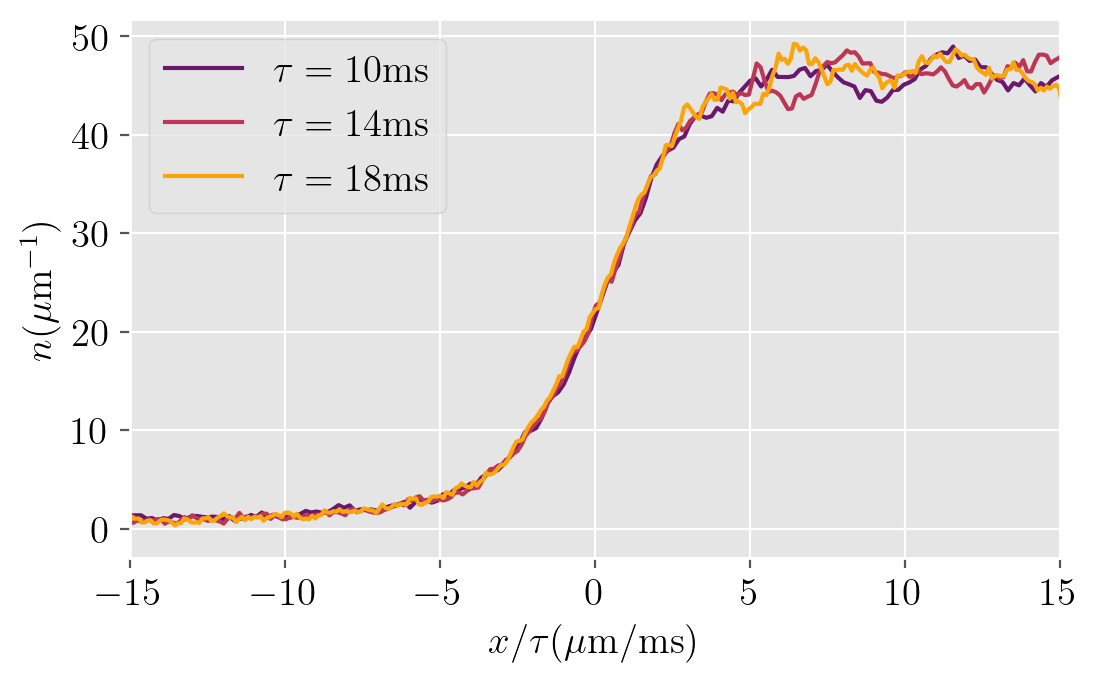
\includegraphics[width=0.7\linewidth]{Figures/Hydroscaling_DWD.png}
    \caption{Caption}
    \label{fig:euler}
\end{figure}



\begin{itemize}
    \item Comparison with the ground state and $\gamma = 6 \times 10^{-3} : $ FIGURE. 
    \item Comparison with the ground state and $\gamma \to 0 : $ FIGURE and conclusion. The edge profile obtained at $T=0$ with $\gamma = 6.10^{-3}$ is nearly identical to the parabola expected at $\gamma \to 0$. The deviations from the parabola observed experimentally are mainly due to non-zero entropy effects. 
\end{itemize}

\textit{Transition : } we would like to extract the rapidiy distribution from the edge profile


\section{Extraction of the initial rapidity distribution}

\subsection{Directly from the edge profile}
{\bf [Premier jet : Jérôme]}
\begin{itemize}
    \item Introducing the Jerôme's method
\end{itemize}

\textit{Transition :} This method is highly sensitive to the linear density away from the edge. Since the signal-to-noise ratio in our experimental data is important in this region, The results obtained with this technique are not trustworthy.

\subsection{Using GHD equations}

\begin{itemize}
    \item Thermal ansatz
    \item Non thermal ansatz
\end{itemize}

We propose to extract the rapidity distribution $\rho (\theta)$ of the initial homogeneous gas by fitting the experimental results with the GHD simulations. 
Extracting $\rho (\theta)$ remains a hard task since we would have an infinite number of fitting parameters $-$ the whole rapidity distribution $-$ with a limited calculation time.
Thus, we have to limit the number of fitting parameters and choose an ansatz for the form of the rapidity distribution.

The first ansatz that we choose is the rapidity distribution for a Gibbs ensemble, the fitting parameters being the temperature $T$ and the chemical potential $\mu$.
%There is \textit{a priori} no reason explaining such a choice  rather than another one, the 1D Bose gas being integrable.


\section{Probing locally the rapidity distribution}
{\bf [Premier jet : Guillaume]}
\label{sec:local}

 \begin{figure}[!htb]
     \centering
     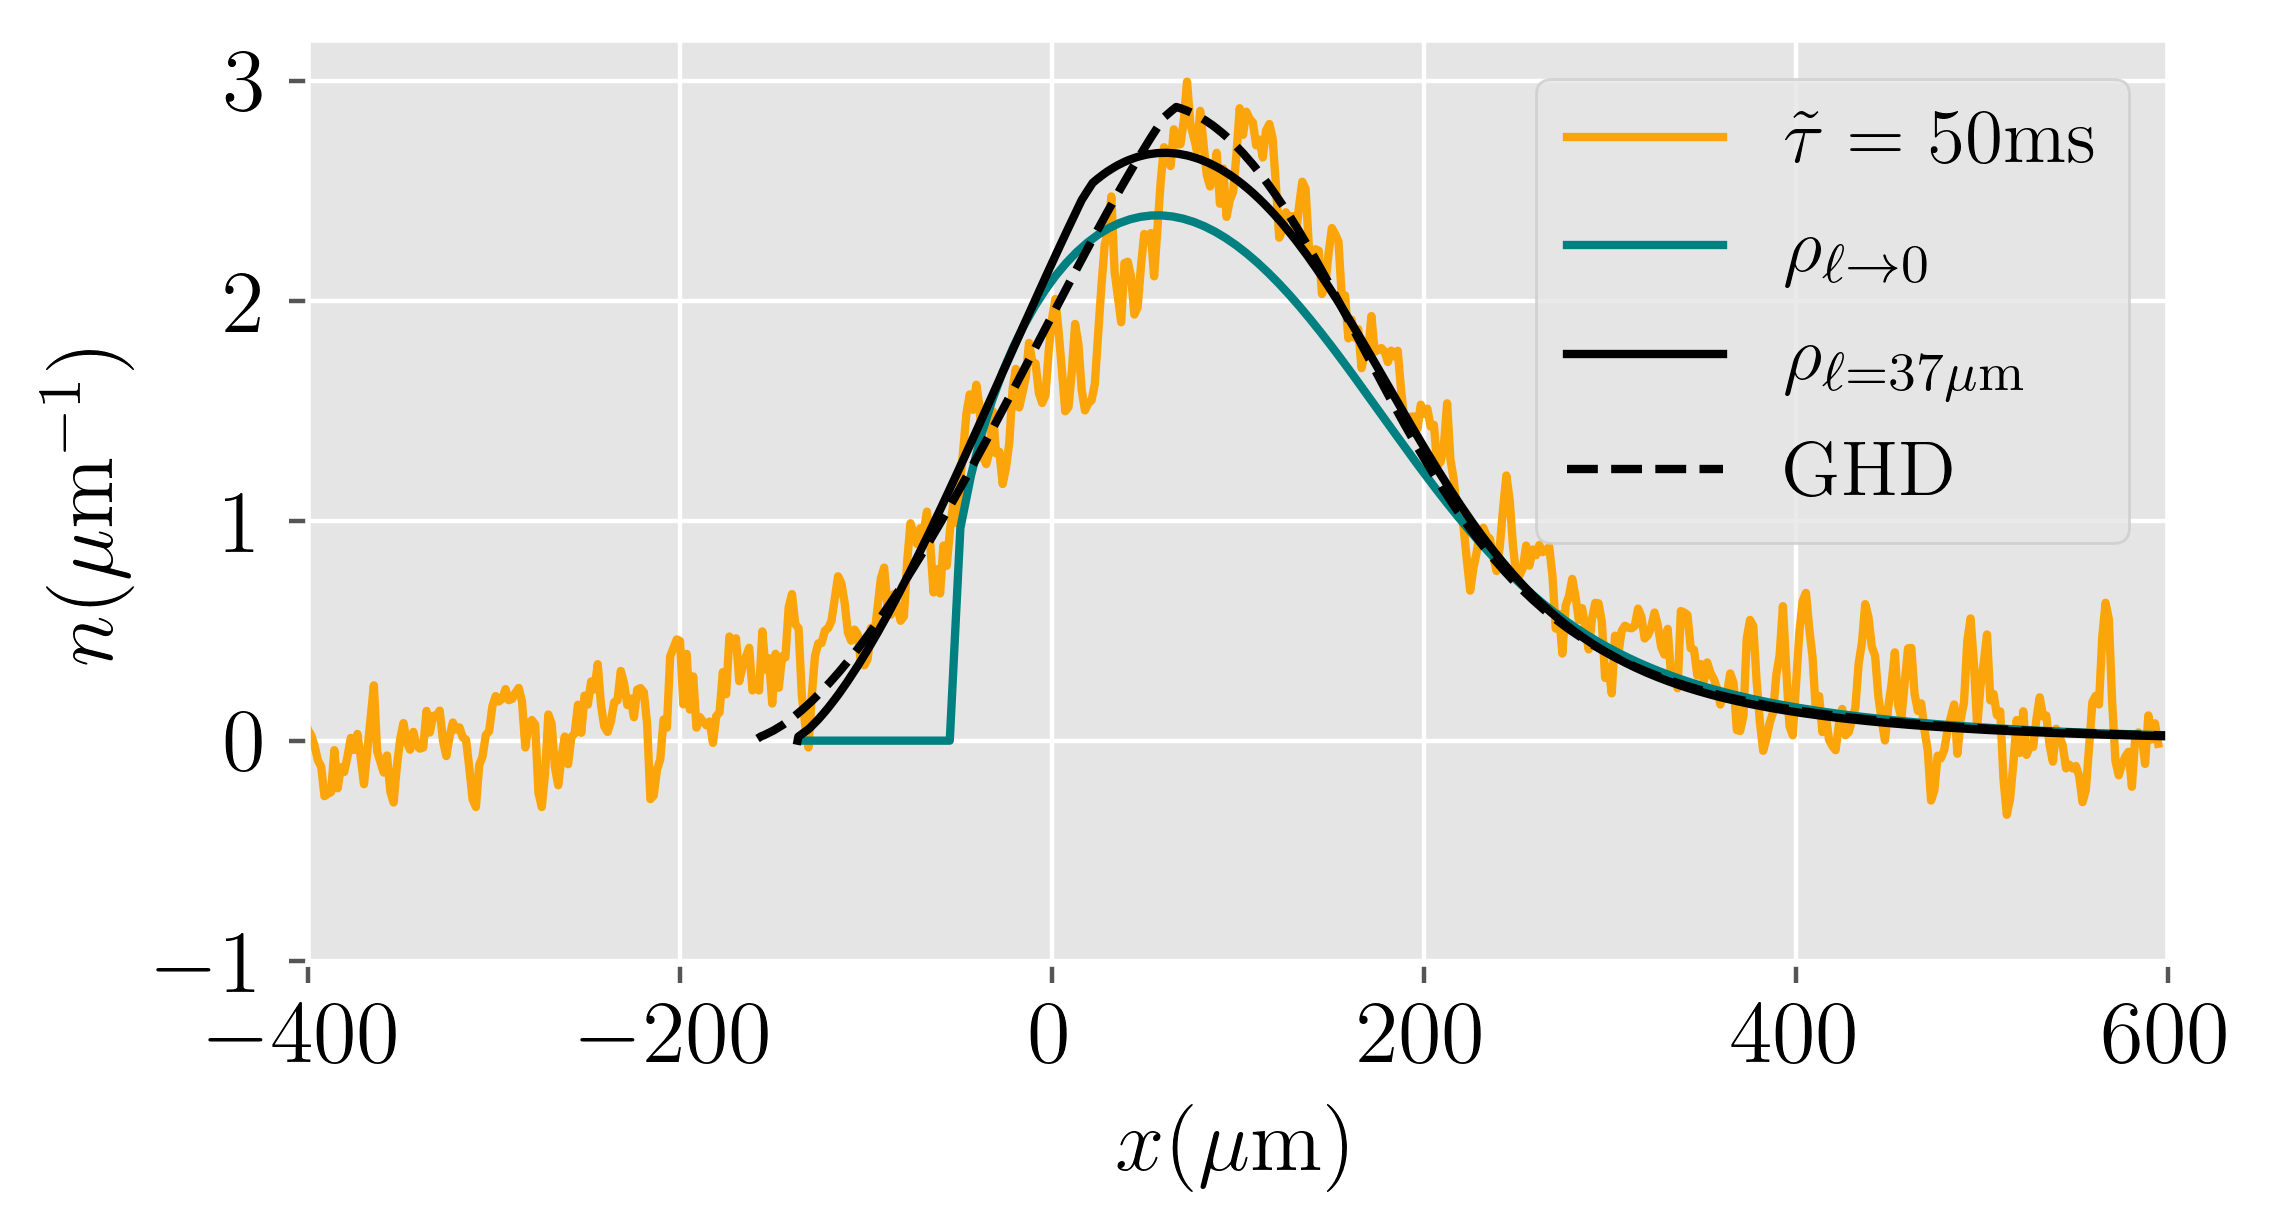
\includegraphics[width=0.8\linewidth]{Figures/asymetrie_GHD_all.png}
     \caption{A second graph for this last part, change the format (.pdf). Add the profile n(-x) to add. Change the captions with using $\Pi$, the extensive rapidity distribution.}
     \label{fig:local}
 \end{figure}

 \begin{itemize}
     \item GHD simulations predict locally a non thermal and asymetric rapidity distribution at the edge deformation. Maybe we can explain technical things about the simulations
     \item Describe the experimental protocol, referring to the previous article.  
     \item Experimental data, profile asymmetry highlighted
     \item First comparison with the assumed homogeneous rapidity distribution in the slice
     \item Second comparison with the inhomogeneous rapidity distribution in the slice
     \item Third comparison with the GHD simulations to take into account the fact that the asymptotic regime is not completely reached.
 \end{itemize}

\section{Conclusion}
\begin{itemize}
    \item a protocol that could enable the study of zero-entropy physics
\end{itemize}

\section*{Acknowledgements}

% \paragraph{Author contributions}
% This is optional. If desired, contributions should be succinctly described in a single short paragraph, using author initials.

\paragraph{Funding information}


% \begin{appendix}

% \section{First appendix}
% Add material which is better left outside the main text in a series of Appendices labeled by capital letters.

% \section{About references}
% Your references should start with the comma-separated author list (initials + last name), the publication title in italics, the journal reference with volume in bold, start page number, publication year in parenthesis, completed by the DOI link (linking must be implemented before publication). If using BiBTeX, please use the style files provided  on \url{https://scipost.org/submissions/author_guidelines}. If you are using our \LaTeX template, simply add
% \begin{verbatim}
% \bibliography{your_bibtex_file}
% \end{verbatim}
% at the end of your document. If you are not using our \LaTeX template, please still use our bibstyle as
% \begin{verbatim}
% \bibliographystyle{SciPost_bibstyle}
% \end{verbatim}
% in order to simplify the production of your paper.
% \end{appendix}


% TODO:
% Provide your bibliography here. You have two options:

% FIRST OPTION - write your entries here directly, following the example below, including Author(s), Title, Journal Ref. with year in parentheses at the end, followed by the DOI number.
%\begin{thebibliography}{99}
%\bibitem{1931_Bethe_ZP_71} H. A. Bethe, {\it Zur Theorie der Metalle. i. Eigenwerte und Eigenfunktionen der linearen Atomkette}, Zeit. f{\"u}r Phys. {\bf 71}, 205 (1931), \doi{10.1007\%2FBF01341708}.
%\bibitem{arXiv:1108.2700} P. Ginsparg, {\it It was twenty years ago today... }, \url{http://arxiv.org/abs/1108.2700}.
%\end{thebibliography}

% SECOND OPTION:
% Use your bibtex library
% \bibliographystyle{SciPost_bibstyle}
\bibliography{Biblio_Lea.bib,Domain_Wall_paper}

\nolinenumbers

\end{document}
